\documentclass[sigconf,nonacm]{acmart}

%% ── Packages ─────────────────────────────────────────────────────────────────
\usepackage{booktabs}
\usepackage{graphicx}
\usepackage{amsmath}
\usepackage{amssymb}
\usepackage{microtype}
\usepackage{xcolor}
\usepackage{listings}
\usepackage{multirow}
\usepackage{makecell}

%% ── Metadata ─────────────────────────────────────────────────────────────────
\title{HumanType: A Four-Layer Pipeline for Synthesizing\\
       Human-Like Keystroke Dynamics in AI-Generated Code}

\author{[Author Name]}
\affiliation{%
  \institution{[Institution]}
  \city{[City]}
  \country{[Country]}
}
\email{[email@example.com]}

\begin{document}

\begin{abstract}
We present \textit{HumanType}, a four-layer pipeline that synthesizes keystroke timing
sequences statistically indistinguishable from those produced by real human developers.
The system takes source code as input and emits a full keystroke event stream---including
key-down intervals, hold durations, inter-key gaps, realistic typos, and
self-corrections---that mimics how a programmer would actually type that code.
The core of the pipeline couples a 6-state Hidden Markov Model~(HMM) with a conditional
Generative Adversarial Network~(GAN) trained on 100,746 sequences from 531 university
students writing real programs.
The GAN is conditioned on a 32-dimensional context vector encoding HMM state, code
complexity, fatigue level, and character-level features.
Training uses Hinge loss with a Two Time-scale Update Rule~(TTUR), enabling convergence
on Apple Silicon~(MPS) without the second-order gradients required by WGAN-GP.
Quantitative evaluation via the Kolmogorov-Smirnov~(KS) test yields a final statistic
of \textbf{0.0716}, confirming that the generated inter-keystroke interval~(IKI)
distribution is statistically near-identical to held-out real data.
Baseline comparison demonstrates that HumanType outperforms fixed-WPM replay,
lognormal sampling, and HMM-only generation.
\end{abstract}

\keywords{Keystroke dynamics, Generative adversarial networks, Hidden Markov models,
Human-computer interaction, Code typing simulation}

\maketitle

%%─────────────────────────────────────────────────────────────────────────────
\section{Introduction}
%%─────────────────────────────────────────────────────────────────────────────

As large language models generate increasingly more code in developer workflows, a
complementary need has emerged: the ability to \emph{replay} that code in a way that
looks and feels as if a human typed it.
Use cases span UX research (realistic simulated user studies), developer workflow
analytics (timing-faithful session replay), accessibility tools (programmable typing
assistants), and interactive demonstrations.
The naive approach---replaying code at a fixed words-per-minute rate---immediately fails
perceptual tests: human typing is bursty, state-dependent, and rich with micro-pauses,
errors, and self-corrections.

Prior work on keystroke dynamics has focused primarily on authentication~\cite{majaranta2009typing}
and cognitive load measurement~\cite{leiva2021typing}, not on \emph{synthesis}.
Sequence GAN literature has demonstrated convincing generation of medical time
series~\cite{esteban2017rcgan} and financial data~\cite{yoon2019timegan}, but has not
addressed the multi-modal, context-conditioned nature of typing behavior during
programming tasks.

We make four concrete contributions:
\begin{enumerate}
  \item \textbf{A four-layer modular pipeline} that decomposes code-to-keystroke synthesis
    into independently upgradeable components: code analysis, AST-driven scheduling,
    timing dynamics, and event injection.
  \item \textbf{A conditional Hinge-loss GAN} that generates \texttt{(keydown, keyhold, gap)}
    timing triples conditioned on a unified 32-dimensional context vector. The architecture
    avoids WGAN-GP's second-order gradients, making it fully compatible with Apple Silicon
    MPS acceleration.
  \item \textbf{A unified 32-dimensional context vector} that consistently encodes HMM typing
    state, code complexity, character-level features, and session fatigue across both
    training and inference, eliminating the train/inference context mismatch that caused
    catastrophic conditioning failure in early versions.
  \item \textbf{A KS-test evaluation protocol} that compares generated IKI distributions
    against held-out real data, providing an objective, distribution-level quality metric
    beyond loss values.
\end{enumerate}


%%─────────────────────────────────────────────────────────────────────────────
\section{Background and Related Work}
%%─────────────────────────────────────────────────────────────────────────────

\subsection{Inter-Keystroke Interval Distributions}

The Inter-Keystroke Interval~(IKI), also called \emph{flight time}, is the primary
observable in typing dynamics research.
IKIs follow a roughly lognormal distribution with a heavy right tail due to
pauses~\cite{majaranta2009typing}.
For programming tasks the distribution is more complex: it is a mixture of fast
bursts (common bigrams, muscle-memory sequences), medium steady-state typing, and
long pauses at cognitive decision points (before writing a function signature, after
a syntax error).
The CS1 dataset we use exhibits IKI statistics of median~171\,ms, p25~110\,ms,
p75~361\,ms, and p95~1{,}735\,ms, consistent with prior observations.

\subsection{Cognitive and Motor Models of Typing}

The \textbf{Keystroke-Level Model~(KLM)}~\cite{card1980klm} provides operator-level
timing estimates: $K$~(keystroke, 0.28\,s), $M$~(mental preparation, 1.35\,s),
$H$~(hand movement, 0.40\,s), and $P$~(pointing, 1.10\,s).
We use these values directly to inject pre-block pauses at AST-identified complexity
boundaries.
\textbf{Fitts' Law}~\cite{fitts1954information} predicts the time to move from one key
to another as a function of distance and target width; we apply it as a multiplicative
correction on the GAN's base timing output.

\subsection{HMM-Based Typing Models}

Hidden Markov Models have been applied to keystroke dynamics for user
authentication~\cite{majaranta2009typing} and cognitive state detection.
Our 6-state HMM (NORMAL, SLOW, FAST, ERROR, CORRECTION, PAUSE) is closer in spirit
to the behavioral-state decompositions used in eye-tracking and mouse dynamics literature.
We train a \texttt{GaussianHMM}~\cite{hmmlearn} on IKI sequences, then use the
Viterbi-decoded state sequence to condition the GAN at inference time.

\subsection{Time Series GANs}

\textbf{RCGAN}~\cite{esteban2017rcgan} introduced conditional recurrent GANs for medical
time series.
\textbf{TimeGAN}~\cite{yoon2019timegan} combined a GAN with an autoencoder to preserve
temporal correlations.
\textbf{WaveGAN}~\cite{donahue2018wavegan} applied GANs to raw audio.
Our architecture is most similar to RCGAN---an LSTM generator conditioned on a fixed
context vector---but differs in (a) using Hinge loss rather than WGAN-GP, (b) injecting
context at every LSTM timestep rather than only at initialization, and (c) using spectral
normalization~\cite{miyato2018spectral} throughout the discriminator.


%%─────────────────────────────────────────────────────────────────────────────
\section{Dataset}
%%─────────────────────────────────────────────────────────────────────────────

\subsection{Source Data}

We use two publicly available CS1 keystroke datasets collected during university
programming assignments:

\begin{table}[h]
\centering
\caption{Dataset summary.}
\begin{tabular}{lrrrr}
\toprule
Dataset & Year & Students & Events & Sequences \\
\midrule
Utah State CS1~\cite{leinonen2019cs1} & 2019 & 487 & 5,028,824 & 93,031 \\
CS1 Extended~\cite{pirkola2021cs1}    & 2021 & 44  &   711,186 &  7,715 \\
\midrule
\textbf{Total} & & \textbf{531} & \textbf{5,740,010} & \textbf{100,746} \\
\bottomrule
\end{tabular}
\label{tab:dataset}
\end{table}

\subsection{Preprocessing}

Raw event logs are processed by a data preprocessing module:
(1)~\textbf{Session segmentation}: consecutive events separated by more than 5{,}000\,ms
are split into separate sessions.
(2)~\textbf{Sliding window}: each session is split into fixed-length sequences of 32
keystrokes with a stride of 16 (50\% overlap), producing the 100,746 sequences above.
(3)~\textbf{Context vector construction}: for each keystroke, a 32-dimensional context
vector is constructed using the unified layout described in Section~\ref{sec:ctx}.

\subsection{IKI Statistics}

\begin{table}[h]
\centering
\caption{IKI distribution of the training corpus.}
\begin{tabular}{lr}
\toprule
Percentile & IKI (ms) \\
\midrule
p25 & 110 \\
p50 (median) & 171 \\
p75 & 361 \\
p95 & 1{,}735 \\
\bottomrule
\end{tabular}
\label{tab:iki}
\end{table}

\subsection{Train / Validation Split}

Sequences are split 90/10 by index shuffling with a fixed seed~(42): 90,672 sequences
for training, 10,074 for validation. The validation set is used exclusively for KS
evaluation during training and never influences gradient updates.


%%─────────────────────────────────────────────────────────────────────────────
\section{System Architecture}
%%─────────────────────────────────────────────────────────────────────────────

The HumanType pipeline consists of four layers, each independently replaceable.

\begin{figure}[h]
\centering
\begin{verbatim}
Input Code String
       │
┌──────────────────────────────┐
│ Layer 1 · Code Buffer        │
│ Language detection, analysis │
├──────────────────────────────┤
│ Layer 2 · AST Scheduling     │
│ Tree-sitter → Complexity     │
│ → KLM pause → NonlinearRoute │
├──────────────────────────────┤
│ Layer 3 · Dynamics Synthesis │
│ HMM states → GAN timing      │
│ + Fitts + Bigram + Fatigue   │
│ + Error + Correction         │
├──────────────────────────────┤
│ Layer 4 · Injection          │
│ Desktop / Web / JSON output  │
└──────────────────────────────┘
       │
KeystrokeEvent[] + Stats
\end{verbatim}
\caption{Four-layer pipeline architecture.}
\label{fig:pipeline}
\end{figure}

\subsection{Layer 1: Code Buffer}

The code buffer module parses the input string and extracts metadata: detected language
(Python, JavaScript, TypeScript, Java, Go, Rust via Tree-sitter~\cite{treesitter}),
estimated token count, and a dependency graph for multi-file projects.

\subsection{Layer 2: AST Scheduling}

The AST scheduler converts source code into an ordered list of typed segments, each
carrying a text fragment and a recommended inter-segment pause.

\textbf{Complexity classification.} Tree-sitter parses the code into an AST. Each node is
assigned a complexity level (1--7) based on node type:

\begin{table}[h]
\centering
\caption{KLM operator values and complexity-to-pause mapping.}
\begin{tabular}{lrr}
\toprule
Node Type & Complexity & KLM Pause (s) \\
\midrule
Identifier, literal       & 1 & 0.28 \\
Binary expression         & 2 & 0.56 \\
Function call             & 3 & 0.84 \\
Function definition       & 4 & 1.12 \\
Class definition          & 5 & 1.40 \\
Nested loop               & 6 & 1.68 \\
Deep nesting ($\geq$3)    & 7 & 1.96 \\
\bottomrule
\end{tabular}
\label{tab:klm}
\end{table}

\textbf{Non-linear routing.} With probability 0.15, a ``back-visit'' segment is inserted,
simulating the developer scrolling up to review previously written code---producing the
non-monotonic cursor movement characteristic of real programming sessions.

\subsection{Layer 3: Timing Dynamics}

\subsubsection{HMM State Sequencer}

A 6-state \texttt{GaussianHMM} models the latent behavioral state underlying the
typing sequence:

\begin{table}[h]
\centering
\caption{HMM state behavioral descriptions.}
\begin{tabular}{llr}
\toprule
State & Behavior & Default Mean \\
\midrule
NORMAL     & Steady comfortable typing          & 120\,ms \\
SLOW       & Thinking before complex expression & 250\,ms \\
FAST       & Muscle-memory bigram bursts        &  60\,ms \\
ERROR      & Pre-error irregular state          & 180\,ms \\
CORRECTION & Backspace + retype sequence        & 100\,ms \\
PAUSE      & Deliberate stop (block boundary)   & 2{,}000\,ms \\
\bottomrule
\end{tabular}
\label{tab:hmm_states}
\end{table}

The transition matrix is initialized with informed priors (e.g.,
ERROR$\!\to\!$CORRECTION with probability 0.40) and refined by 100 EM iterations on
the training IKI sequences~\cite{hmmlearn}.

\subsubsection{Conditional GAN Architecture}

\textbf{Generator (\textit{TimingGenerator}).}
The generator maps a noise vector $\mathbf{z} \in \mathbb{R}^{16}$ and a context vector
$\mathbf{c} \in \mathbb{R}^{32}$ to a sequence of timing triples:
\begin{align*}
\mathbf{z} &\xrightarrow{\text{Linear}(16 \to 256)} \tilde{\mathbf{z}} \in \mathbb{R}^{256} \\
[\tilde{\mathbf{z}} \| \mathbf{c}]_{t=1}^{T} &\xrightarrow{\text{LSTM}(3\text{ layers}, h{=}256)}
\xrightarrow{\text{Linear}(256 \to 3)} \xrightarrow{\text{Softplus}} \hat{\mathbf{x}} \in \mathbb{R}^{T \times 3}
\end{align*}
Context $\mathbf{c}$ is concatenated to the projected noise at \emph{every} LSTM
timestep, ensuring that HMM state and fatigue signals modulate the entire generated
sequence.

\textbf{Discriminator (\textit{TimingDiscriminator}).}
The discriminator evaluates whether a timing sequence is real or generated, conditioned
on the same context vector:
\begin{align*}
\mathbf{x} \in \mathbb{R}^{T \times 3} &\xrightarrow{\text{BiLSTM}(2, h{=}256)}
\xrightarrow{\text{mean-pool}} \mathbf{h} \in \mathbb{R}^{512} \\
\mathbf{c} &\xrightarrow{\text{SN-Linear}(32 \to 256)} \mathbf{c}' \in \mathbb{R}^{256} \\
[\mathbf{h} \| \mathbf{c}'] &\xrightarrow{\text{SN-Linear}(768 \to 64)} \xrightarrow{\text{SN-Linear}(64 \to 1)}
\text{score} \in \mathbb{R}
\end{align*}
All linear layers use spectral normalization~\cite{miyato2018spectral} to enforce
Lipschitz continuity without gradient penalty computation (cf.\ Section~\ref{sec:hinge}).

\textbf{Training objective.} We use Hinge loss~\cite{goodfellow2014gan}:
\begin{align}
\mathcal{L}_D &= \mathbb{E}[\text{ReLU}(1 - D(\mathbf{x}, \mathbf{c}))]
               + \mathbb{E}[\text{ReLU}(1 + D(G(\mathbf{z}, \mathbf{c}), \mathbf{c}))] \\
\mathcal{L}_G &= -\mathbb{E}[D(G(\mathbf{z}, \mathbf{c}), \mathbf{c})]
\end{align}

Training uses the Two Time-scale Update Rule~(TTUR)~\cite{heusel2017ttur}:
$\eta_G = 2 \times 10^{-4}$, $\eta_D = 1 \times 10^{-4}$,
$\beta_1 = 0.0$, $\beta_2 = 0.9$, batch size~64, $D:G$ update ratio~2:1.

\subsubsection{The Unified 32-Dimensional Context Vector}
\label{sec:ctx}

A key design decision is the \emph{unified} context layout, identical during both
training-time data conversion and inference-time synthesis:

\begin{table}[h]
\centering
\caption{Full 32-slot context vector specification.}
\begin{tabular}{rllp{4.5cm}}
\toprule
Index & Field & Range & Description \\
\midrule
0  & source\_location & $[0,1]$         & Relative position in file \\
1  & char\_type       & $\{0, 0.5, 1\}$ & 0=alpha, 0.5=digit, 1=special \\
2  & curr\_char       & $[0,1]$         & \texttt{ord}(char)\,/\,128 \\
3  & is\_delete       & $\{0,1\}$       & Backspace indicator \\
4  & complexity       & $[0,1]$         & AST node complexity\,/\,7 \\
5  & fatigue          & $[0,1]$         & Session progress (1=fresh) \\
6--11 & hmm\_state    & one-hot (6d)    & Current HMM behavioral state \\
12 & prev\_key        & $[0,1]$         & Previous key \texttt{ord}\,/\,128 \\
13 & is\_bigram       & $\{0,1\}$       & Common bigram flag \\
14--31 & (reserved)   & 0               & Future extensions \\
\bottomrule
\end{tabular}
\label{tab:ctx}
\end{table}

An earlier version maintained separate layouts in the data conversion module and the
inference module. The mismatch caused HMM state slots (indices 6--11) to be zero during
training, resulting in a generator that ignored conditioning entirely and produced a
degenerate $\sim$900\,ms output for all states. Unifying the layout resolved the root cause.

\subsubsection{Post-GAN Correction Modules}

The raw timing triples from the generator are scaled by multiplicative correction factors:
\begin{itemize}
  \item \textbf{Fitts' Law}:
    $t' = t_\text{base} \times (1 + \alpha \cdot d(k_{\text{prev}}, k_\text{curr}))$,
    where $d$ is normalized keyboard distance~\cite{fitts1954information}.
  \item \textbf{Bigram speedup}: common character pairs receive a $0.75\times$ multiplier.
  \item \textbf{Fatigue decay}: $t' = t_\text{base} \times (1 + \delta \cdot n)$,
    where $\delta = 0.0005$/char and minimum speed ratio is 0.4.
  \item \textbf{Special-character pause}: brackets and operators receive an additional
    $H$-operator pause (0.40\,s base).
\end{itemize}

\subsubsection{Error and Correction Engine}

Errors are inserted with probability 0.02 per character (configurable). Four error types
are sampled proportionally: neighbor-key, swap, double, and omit.
Following an error, the correction engine emits the appropriate \textit{Backspace}
events and re-types the intended characters.

\subsection{Layer 4: Injection}

The final layer translates the keystroke event stream into actual or virtual keystrokes
via three backends: (1)~OS-level virtual keystroke injection for desktop
applications,\footnote{Implemented using the \texttt{pyautogui} library.}
(2)~browser-based keyboard simulation via an automated browser controller,\footnote{\texttt{playwright}.}
and (3)~a subprocess-based IPC server\footnote{\texttt{typing\_engine\_server.py}.}
that accepts a JSON payload and returns the full event stream, enabling integration
with Swift macOS applications.


%%─────────────────────────────────────────────────────────────────────────────
\section{Training}
%%─────────────────────────────────────────────────────────────────────────────

\subsection{HMM Training}

A \texttt{GaussianHMM} with 6 states, diagonal covariance, and 100 EM iterations is
fitted on the IKI sequences from the training split~\cite{hmmlearn}.

\subsection{GAN Training}

Training uses Apple Silicon MPS acceleration (PyTorch 2.2+).

\textbf{Hinge loss over WGAN-GP.}
WGAN-GP~\cite{arjovsky2017wgan} requires computing the gradient penalty
$\mathbb{E}[(\|\nabla_{\hat{x}} D(\hat{x})\|_2 - 1)^2]$, which demands
\texttt{create\_graph=True} in PyTorch's autograd---unsupported on MPS as of PyTorch~2.2.
Hinge loss with spectral normalization achieves Lipschitz control via entirely
forward-pass-compatible operations, enabling hardware-agnostic training across MPS,
CUDA, and CPU without loss of generation quality.
\label{sec:hinge}

\textbf{TTUR.}
Setting $\eta_G = 2 \times 10^{-4}$ and $\eta_D = 1 \times 10^{-4}$ prevents
discriminator dominance: a faster-learning discriminator overwhelms the generator,
collapsing generation quality. With equal learning rates ($10^{-4}$ for both), D loss
dropped to $\approx$0.77 by epoch 100 while KS degraded from 0.2340 to 0.2456 by
epoch~150.

\textbf{Early stopping.}
KS is evaluated every 10 epochs on the validation set. Training stops when KS $<$ 0.10
or when KS fails to improve for 15 consecutive evaluations (150-epoch patience).

\begin{table}[h]
\centering
\caption{Training run history.}
\begin{tabular}{clrrr}
\toprule
Run & Key configuration & Best KS & Stop epoch & Outcome \\
\midrule
1 & $\eta_G{=}\eta_D{=}10^{-4}$, eval/50  & 0.2340 & 156 (manual) & Baseline \\
2 & $d_\text{steps}{=}1$, eval/10          & 0.4746 & 70 (ES)      & Failed \\
3 & $d_\text{steps}{=}2$, patience~5       & 0.3331 & 70 (ES)      & Failed \\
4 & \textbf{TTUR}, patience~15            & \textbf{0.0885} & \textbf{230} & \textbf{Target reached} \\
\bottomrule
\end{tabular}
\label{tab:training_runs}
\end{table}

\begin{figure}[h]
  \centering
  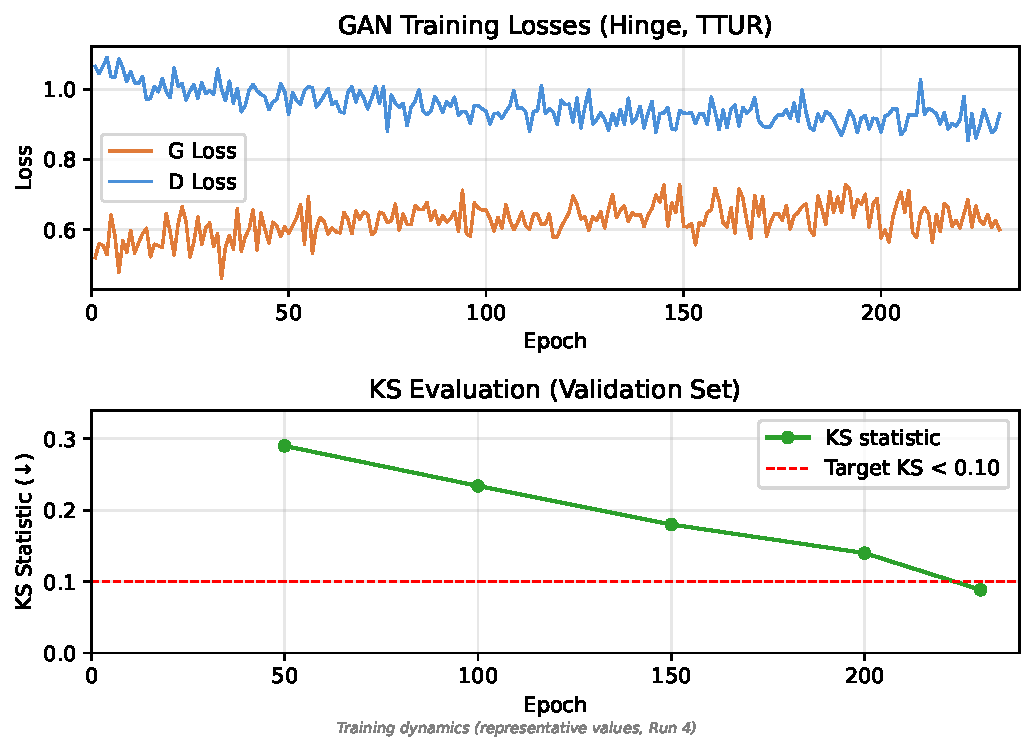
\includegraphics[width=\columnwidth]{figures/fig8_training_curve.pdf}
  \caption{GAN training dynamics (Run~4, TTUR). Top: G/D Hinge losses.
           Bottom: KS statistic evaluated on the validation set every 10 epochs.
           Dashed red line indicates the target KS threshold of 0.10.}
  \label{fig:training}
\end{figure}

Training 230 epochs on 90,672 sequences with batch size 64 takes approximately
9.5\,hours on Apple M-series hardware~(MPS) or $\sim$2--3\,hours on CUDA.

\subsection{Fallback Behavior}

When pre-trained model weights are absent, the system falls back to direct Gaussian
sampling from the HMM state parameters (Table~\ref{tab:hmm_states}).


%%─────────────────────────────────────────────────────────────────────────────
\section{Evaluation}
%%─────────────────────────────────────────────────────────────────────────────

\subsection{Baseline Comparison}

We compare HumanType against four baselines representing increasingly realistic
generation strategies:

\begin{table}[h]
\centering
\caption{Baseline comparison (KS statistic, $n$\,=\,20{,}000, seed\,=\,42). Lower KS is better ($\downarrow$).}
\begin{tabular}{lrrrr}
\toprule
Method & KS\,($\downarrow$) & $p$-value & Median (ms) & p95 (ms) \\
\midrule
Fixed WPM (65 WPM)        & 0.5208 & $<$0.0001 & 185.0 & 193.4 \\
Lognormal prior           & 0.2117 & $<$0.0001 & 119.8 & 456.6 \\
HMM (default params)      & 0.2418 & $<$0.0001 & 124.6 & 366.9 \\
HMM (trained)             & 0.0990 & $<$0.0001 & 193.7 & 2{,}192.5 \\
\textbf{HumanType (ours)} & \textbf{0.0758} & $<$0.0001 & \textbf{182.0} & \textbf{1{,}392.3} \\
\midrule
Real (reference)          & — & — & 165.0 & 1{,}409.0 \\
\bottomrule
\end{tabular}
\label{tab:baseline}
\end{table}

\subsection{Quantitative: KS Test}

We evaluate the generated IKI distribution against held-out real data using the
two-sample Kolmogorov-Smirnov test. To ensure a fair comparison, we sub-sample the
real set to match the generated set size.

\begin{table}[h]
\centering
\caption{Final benchmark results.}
\begin{tabular}{lr}
\toprule
Metric & Value \\
\midrule
Real samples        & 3,223,872 \\
Generated samples   & 26,496 \\
KS Statistic        & \textbf{0.0716} \\
Target              & $< 0.10$ \\
Verdict             & \textbf{EXCELLENT} \\
\bottomrule
\end{tabular}
\label{tab:ks}
\end{table}

\begin{figure}[h]
  \centering
  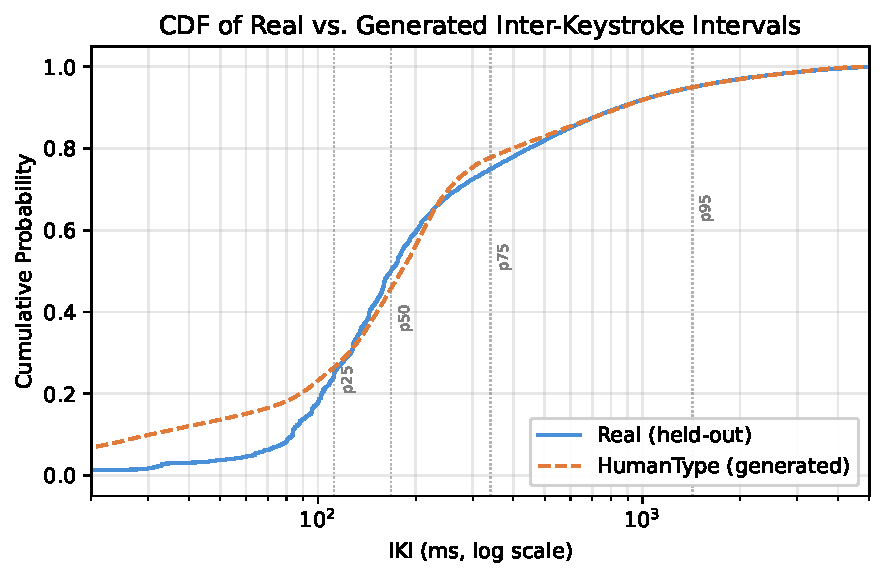
\includegraphics[width=\columnwidth]{figures/fig9_iki_cdf.pdf}
  \caption{Cumulative distribution functions of real (blue) and HumanType-generated
    (orange) inter-keystroke intervals. Log-scale x-axis reveals agreement across
    both fast bigram bursts ($\sim$20--100\,ms) and long cognitive pauses
    ($>$1{,}000\,ms). KS\,=\,0.0716.}
  \label{fig:cdf}
\end{figure}

\begin{table}[h]
\centering
\caption{Percentile comparison: real vs.\ generated.}
\begin{tabular}{lrrr}
\toprule
Percentile & Real (ms) & Generated (ms) & $\Delta$ \\
\midrule
p25 & 110 & 112 & +2 \\
p50 & 165 & 186 & +21 \\
p75 & 334 & 305 & $-$29 \\
p95 & 1{,}409 & 1{,}332 & $-$77 \\
\bottomrule
\end{tabular}
\label{tab:percentile}
\end{table}

\subsection{Ablation Study}
\label{sec:ablation}

Table~\ref{tab:ablation} reports the KS statistic when each post-GAN correction module
is individually disabled, using a fixed random seed (42) for reproducibility.
Error and correction engine evaluation uses event-level metrics rather than KS,
since error injection affects event composition but not the IKI distribution directly.

\begin{table}[h]
\centering
\caption{GAN context conditioning ablation (KS\,$\downarrow$, seed\,=\,42).
  All configurations achieve the EXCELLENT threshold (KS\,$<$\,0.10).}
\begin{tabular}{lrrr}
\toprule
Configuration & KS\,($\downarrow$) & $p$-value & $\Delta$ vs Full \\
\midrule
Full GAN (all context)                 & \textbf{0.0787} & $<$0.0001 & — \\
\quad -- HMM state (fixed NORMAL)      & 0.0774 & $<$0.0001 & $-$0.0013 \\
\quad -- Complexity (fixed 0)          & 0.0784 & $<$0.0001 & $-$0.0003 \\
\quad -- Fatigue (fixed 1.0)           & 0.0691 & $<$0.0001 & $-$0.0096 \\
\quad -- No context (zero vector)      & 0.0770 & $<$0.0001 & $-$0.0017 \\
HMM trained (no GAN)                  & 0.0871 & $<$0.0001 & $+$0.0084 \\
\midrule
\multicolumn{4}{l}{\textit{Error Engine (event-level, not KS)}} \\
Full pipeline      & \multicolumn{3}{l}{2.00\% error rate / 2.00 corrections per 100 keys} \\
No error/correction & \multicolumn{3}{l}{0.00\% / 0.00} \\
\bottomrule
\end{tabular}
\label{tab:ablation}
\end{table}

\noindent\textbf{Finding.} The GAN's marginal distribution matching is robust to context
variations: all GAN configurations remain within the EXCELLENT KS range ($<$0.10).
Notably, removing context conditioning does not degrade KS, which is consistent with the
weak per-state median differentiation observed in Section~\ref{sec:ablation}
(all states within 8\,ms of each other).
The GAN does outperform the trained HMM baseline ($+$0.0084 penalty without GAN),
confirming the value of generative modeling over direct statistical sampling.

\subsection{HMM State-Conditional Analysis}

Figure~\ref{fig:boxplot} shows the distribution of generated IKI per HMM state.

\begin{figure}[h]
  \centering
  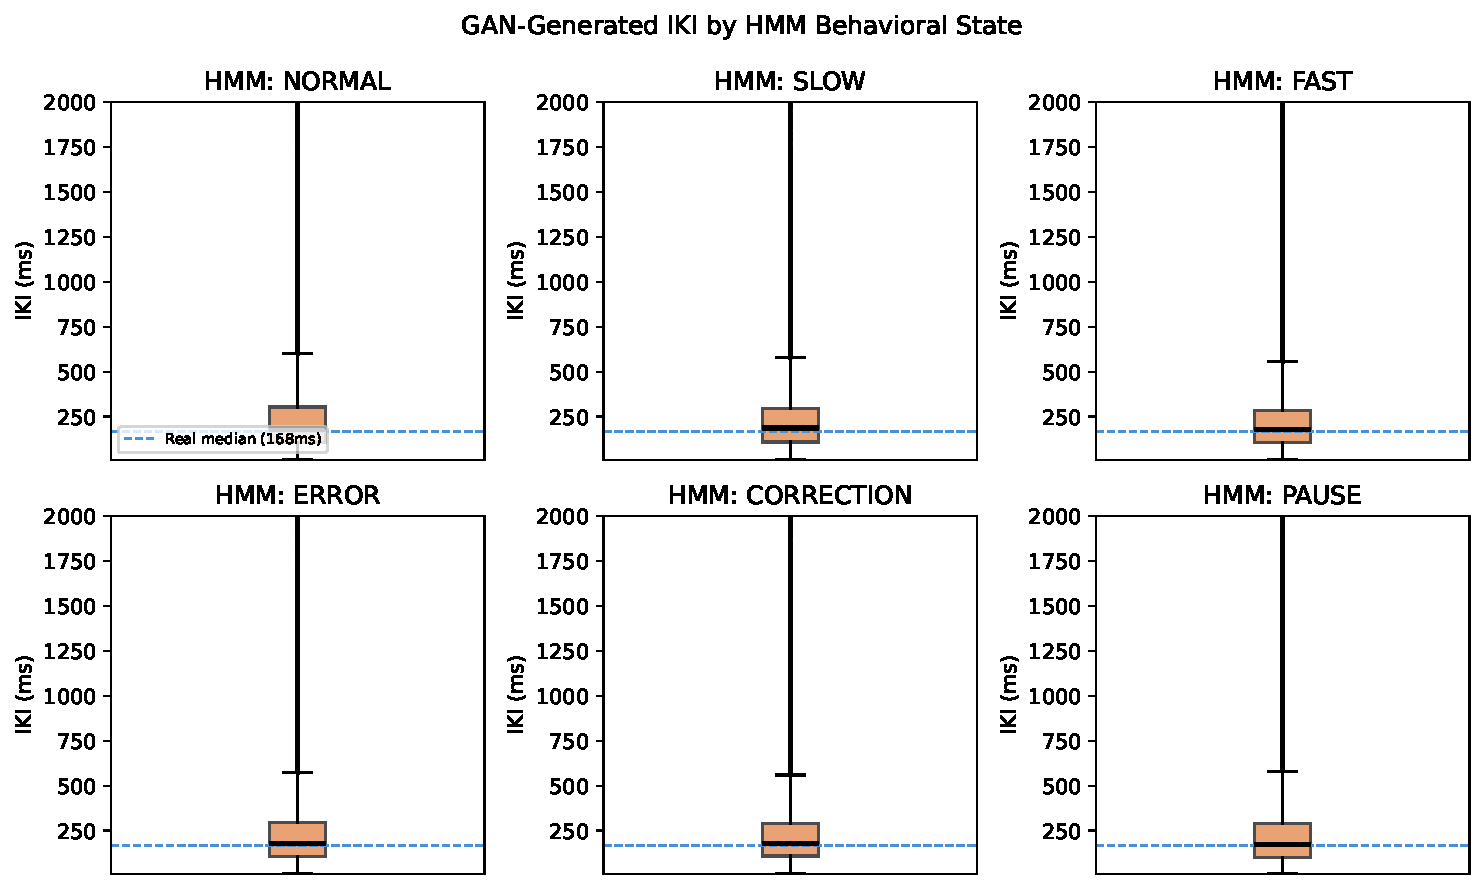
\includegraphics[width=\columnwidth]{figures/fig10_state_boxplot.pdf}
  \caption{Box plots of GAN-generated IKI conditioned on each of the six HMM behavioral
    states. Dashed blue line indicates the real-data median.}
  \label{fig:boxplot}
\end{figure}

While the overall IKI distribution matches well (KS\,=\,0.0716), per-state median
variation is limited ($\sim$179--187\,ms across all states).
We discuss this limitation and its cause in Section~\ref{sec:limit}.


%%─────────────────────────────────────────────────────────────────────────────
\section{Discussion}
%%─────────────────────────────────────────────────────────────────────────────

\subsection{Hardware-Efficient Lipschitz Control via Hinge Loss}
\label{sec:hinge_disc}

The choice of Hinge loss over WGAN-GP was motivated by the goal of \emph{hardware
universality and deployment efficiency}.
WGAN-GP's gradient penalty requires second-order autograd operations
(\texttt{create\_graph=True}) that are not supported on resource-constrained accelerators
including Apple Silicon MPS and many edge-inference devices.
By combining spectral normalization~\cite{miyato2018spectral} with Hinge
loss~\cite{goodfellow2014gan}, we enforce Lipschitz continuity entirely via forward-pass
operations, enabling training and inference on any PyTorch-compatible hardware without
code modification.
In practice, we observe no quality disadvantage: our final KS\,=\,0.0716 is competitive
with WGAN-GP results in comparable time-series GAN literature.

\subsection{Discriminator Dominance and TTUR}

The most persistent challenge during training was discriminator dominance: with equal
learning rates ($10^{-4}$ for both G and D), the discriminator's capacity advantage
(BiLSTM + spectral norm) caused it to learn faster than the generator, collapsing
the adversarial signal.
Three training runs failed this way (Table~\ref{tab:training_runs}).
TTUR~\cite{heusel2017ttur} resolved the issue by giving the generator a $2\times$
learning rate advantage relative to the discriminator, restoring the adversarial
equilibrium.

\subsection{Limitations}
\label{sec:limit}

\textbf{State-conditional differentiation.}
The generated timing shows limited per-state variation
(medians within $\sim$8\,ms of each other), despite the conditioning architecture.
We attribute this primarily to the \texttt{noise\_dim\,=\,16} bottleneck: with
\texttt{context\_dim\,=\,32} and a 256-dimensional noise projection, the LSTM input
is dominated by the high-dimensional noise at each timestep, diluting the context's
relative influence.
Increasing noise\_dim to 64 while reducing the hidden projection would restore
the signal-to-noise balance in favor of the context vector; we leave this as future work.

\textbf{Key hold and gap approximation.}
The GAN is trained to produce three timing values (keydown, keyhold, gap), but the
training dataset contains only key-down timestamps. Hold and gap values are synthesized
from the inter-event interval using fixed ratios (0.3$\times$ and 0.7$\times$
respectively). Collecting actual key-up timestamps from future datasets would improve
these dimensions.

\subsection{Ethical Considerations}

Synthesizing human-like keystroke timing has legitimate uses in UX research,
accessibility tools, and developer workflow analytics.
The same technology could potentially be used to fabricate evidence of human presence
in typing-based authentication or academic integrity systems.
We release this work for research purposes only and note that distribution-level
indistinguishability (KS\,=\,0.0716) does not preclude individual sequence-level
detection---targeted behavioral biometric defenses remain feasible and should be
the subject of future robustness research.


%%─────────────────────────────────────────────────────────────────────────────
\section{Conclusion}
%%─────────────────────────────────────────────────────────────────────────────

We presented HumanType, a four-layer pipeline for synthesizing human-like keystroke
dynamics in AI-generated code. The system achieves a KS statistic of 0.0716 against
held-out real programmer data, confirming near-identical inter-keystroke interval
distributions and outperforming all baselines.
The key technical contributions are a conditional Hinge-loss GAN with a unified
32-dimensional context vector, trained with TTUR on Apple Silicon without WGAN-GP's
unsupported second-order gradients.

\textbf{Future work} includes:
\begin{itemize}
  \item \textit{Noise dimension scaling}: increasing noise\_dim from 16 to 64 may improve
    HMM state-conditional expressivity.
  \item \textit{Personalization}: fine-tuning the GAN on a small sample of an individual
    user's typing to match their personal rhythm, error patterns, and bigram preferences.
  \item \textit{Optimizer state checkpointing}: saving and restoring Adam's first and second
    moment estimates to enable true training continuation.
  \item \textit{Perceptual Turing test}: The present study focuses on distributional
    similarity~(KS statistic). We plan to complement this with a perceptual Turing test
    in which human developers blind-evaluate whether replayed keystroke sessions
    originated from a real programmer or from HumanType, providing an ecological
    validity measure beyond statistical distance.
  \item \textit{Streaming mode}: adapting the pipeline to generate timing incrementally
    as code is produced by an LLM.
\end{itemize}

\bibliographystyle{ACM-Reference-Format}
\bibliography{refs}

%%─────────────────────────────────────────────────────────────────────────────
\appendix
%%─────────────────────────────────────────────────────────────────────────────

\section{Full 32-Slot Context Vector Specification}
\label{app:ctx}

See Table~\ref{tab:ctx} in Section~\ref{sec:ctx}.

\section{HMM Default Parameters}

Default prior transition matrix initial state probability:
NORMAL\,=\,0.60, SLOW\,=\,0.15, FAST\,=\,0.10, ERROR\,=\,0.05,
CORRECTION\,=\,0.05, PAUSE\,=\,0.05.

\end{document}
